\section{Algoritmos}
\label{sec:algoritmos}
O foco principal dos algoritmos utilizados neste trabalho, que serão apresentados a seguir, é obter o máximo de informação dos dados, a fim de construir um modelo, uma arquitetura de Rede Neural, capaz de prever o comportamento do valor do preço do Bitcoin. Os algoritmos utilizados são: \emph{Backpropagation} (para adaptação dos parâmetros) e o $K$-Fold (para seleção de modelo), os quais serão apresentados a seguir.
 
\subsection{Backpropagation}
\label{subsec:backpropagation}

 As Redes Neurais estão entre os algoritmos de aprendizado mais poderosos da atualidade. Um dos grandes desafios das Redes Neurais é a escolha dos parâmetros da rede que maximizam o seu desempenho. A escolha dos parâmetros está relacionada diretamente com a \textbf{função custo}.
 
 Para descrever a função custo, vamos considerar o problema de classificação binária, que é o foco deste trabalho. Do ponto de vista da Rede Neural, ela deve possuir apenas um neurônio na última camada para produzir um valor que será encaixado entre 0 e 1, que é alcançado graças a uma função de ativação (nesse trabalho a função sigmoide foi a adotada).
 
 A função custo utilizada neste trabalho foi a MSE. O Backprogation será usado então para minimizar o resultado da função custo, escolhendo os parâmetros da rede que satisfazem essa condição \cite{lehmann2006theory, werbos1974beyond, Rojas1996, werbosBackpropagationthroughtime}. O Backpropagation tem esse nome porque a atualização dos parâmetros se dá num passo final, o qual calcula os erros do passo anterior (ou passo \textit{forward}) de modo retroativo.
 
 Assim, a primeira parte para calcular o Backpropagation consiste na execução o chamado \textit{forward propagation}, etapa que consiste no cômputo da saída $\mathbf{h_\theta}$. Com a saída $\mathbf{h_\theta}$ calculada, devemos calcular o $\mathbf{\delta_k}$, que é o vetor com todos os erros da camada $k$. O cálculo de $\mathbf{\delta_k}$ pode ser visto na Eq. \eqref{eq:deltak}, que pode ser entendido simplesmente como a subtração da saída esperada,  $\mathbf{y}$, pelo resultado obtido, $\mathbf{a_k}$ (é importante notar que $\mathbf{a_k} = \mathbf{h_\theta}$). 
 
\begin{equation}
\label{eq:deltak}
\mathbf{\delta_k} = \mathbf{a_k} - \mathbf{y}
\end{equation}

Com $\mathbf{\delta_k}$ calculado, regredimos uma camada e calculamos $\mathbf{\delta_{k-1}}$, como mostra a Eq. \eqref{eq:deltak-1}, onde $\mathbf{g'(z^k)}$ pode ser calculado usando a Eq. \eqref{eq:glinha}.

\begin{equation}
\label{eq:deltak-1}
\mathbf{\delta_{k-1}} = (\Theta^{k-1})^T \delta^{k}  \mathbf{g'(z^k)}
\end{equation}
  
\begin{equation}
\label{eq:glinha}
\mathbf{g'(z^k)} = \mathbf{a^{k-1}(1-a^{k-1})}
\end{equation}

Esse procedimento é repetido para todas as $k$ camadas, menos a primeira, que é a camada de entrada, para a qual não faz sentido calcular o erro. A Eq. \ref{eq:deltakgenerico} exemplifica o cálculo dos $\mathbf{\delta_{i}}$, os quais serão usados para atualizar os pesos da Rede Neural.  

\begin{equation}
\label{eq:deltakgenerico}
\mathbf{\delta_{i}} = (\Theta^{i})^T \delta^{i+1}  \mathbf{g'(z^i+1)}.
\end{equation}
 
 Essa é a ideia central do Algoritmo Backpropagation, o qual começa por calcular o erro do final (o mais fácil de ser calculado), para então voltar à primeira camada da rede, atualizando os pesos. Com isso, os pesos são atualizados de sorte a melhor se aproximar do resultado desejado. O Algoritmo \ref{alg:BP} descreve o  Backpropagation de modo completo.
 
 \begin{algorithm}[H]
   \SetAlgoLined
   \Entrada{$\mathbf{X, Y}$} 
   \Saida{$\Theta$}
   \Inicio{
    $   \Delta^{(l)}_{ij} \coloneqq \mathbf{0} $\\
       \Para{i = 1 ; m}{
    $         a^{(1)} \coloneqq x^{1}$\\
            Execute forward propagation $a^{(l)}$ para $l=2,3,...,L $\\
    $        \delta^{(L)} \coloneqq a^{(L)}-y^{(i)} $\\
            Calcule todos os $\delta^{(L-1)}$,$\delta^{(L-1)}$,...,$\delta^{(2)} $\\
    $         \Delta^{(l)}_{ij} \coloneqq \Delta^{(l)}_{ij} + a^{(l)}_{j}\Delta^{(l+1)}_{i} $\\
             \Se{j=0}{
    $         \mathbf{D^{(l)}_{ij}} \coloneqq \frac{1}{m}\Delta^{(l)}_{ij} $\\
             }\Se{j$\neq$0}{
    $          \mathbf{D^{(l)}_{ij}} \coloneqq \frac{1}{m} \Delta^{(l)}_{ij}+\lambda\Theta^{(l)}_{ij} $\\
             }
        }
    $    \Theta = \Theta - \mathbf{D}*a $\\
  }
   \Retorna{$\Theta$}
   \label{alg:BP}
   \caption{\textsc{Algoritmo do Backpropagation }}
 \end{algorithm}

Na próxima seção será abordado um dos métodos utilizados para a seleção de modelos, o $K$-Fold. A adoção deste método é imperiosa, para que a arquitetura da rede escolhida seja robusta e menos propensa ao sobreajuste.

\subsection{\textit{K}-Fold}
 
 Um dos problemas encontrados em soluções de Redes Neurais é a estimativa de quantos Neurônios a Rede terá, visto que não existe na literatura um teorema que diga qual o modelo ideal para cada tipo de problema. Ou seja, trata-se essencialmente de uma escolha empírica. Para ajudar na escolha do modelo de rede, foi usado o algoritmo $K$-fold, que é um algoritmo de validação cruzada que tem como objetivo ajudar a estimar parâmetros do modelo final usando os dados de treino disponíveis \cite{bengio2004no, kohavi1995study, rodriguez2010sensitivity, moreno2012study}.
 
  Para executar o $K$-fold, é preciso primeiro selecionar a quantidade de dados que serão reservados para teste e a quantidade de dados que serão reservados para treinamento do modelo, onde usualmente a escolha gira entre algo em torno de 20\% dos dados disponíveis para teste e 80\% dos dados disponíveis para treinamento. Cumpre notar que este conjunto de teste não se confunde com o conjunto de teste final, o qual sempre será separado do conjunto de treinamento, sendo reservado para a avaliação final de desempenho do modelo neural.
  
  Com os dados de treinamento selecionados, é preciso escolher um número $K \in \mathbb{N}$. Nesse projeto, o número 10 foi escolhido pois, como mostrado no estudo realizado pelo trabalho \cite{kohavi1995study}, $K$=10 é a melhor escola para seleção de modelo. Como $K=10$, os dados de treino devem ser divididos em 10 partes iguais, de modo aleatório. Cada uma dessas partes é chamada de um \textit{fold}. Assim, uma parte entre os $K$-folds é selecionada e reservada. A rede é treinada com os $K-1$ folds restantes e validada com a parte escolhida no inicio. O procedimento é repetido para todos os $K$-folds, onde sempre é armazenado o valor da acurácia e do desvio padrão de cada \textit{fold} usado como validação. A ideia central é que o $K$-fold deve ser executado variando o número de neurônios na rede até um valor definido, onde o modelo de rede escolhido será o que obtiver o menor desvio padrão ou a maior acurácia, ao longo de todos os $K$ \textit{folds}.
  
  \begin{figure}
    \centering
    \caption[Exemplo do $K$-fold]{Exemplo do $K$-fold com $K$=10}
    \label{fig:k-fold}

    \begin{tikzpicture}
        \matrix (M) [matrix of nodes,
            nodes={minimum height = 10mm, minimum width = 1.2cm, outer sep=0, anchor=center, draw},
            column 1/.style={nodes={draw=none}, minimum width = 1.2cm},
            row sep=1mm, column sep=-\pgflinewidth, nodes in empty cells,
            e/.style={fill=black!25}
          ]
          {
            Experimento 1  & |[e]| & & & & & & & & & \\
            Experimento 2  & & |[e]| & & & & & & & & \\
            Experimento 3  & & & |[e]| & & & & & & & \\
            Experimento 4  & & & & |[e]| & & & & & & \\
            Experimento 5  & & & & & |[e]| & & & & & \\
            Experimento 6  & & & & & & |[e]| & & & & \\
            Experimento 7  & & & & & & & |[e]| & & & \\
            Experimento 8  & & & & & & & & |[e]| & & \\
            Experimento 9  & & & & & & & & & |[e]| & \\
            Experimento 10 & & & & & & & & & & |[e]| \\
          };
          \draw (M-1-2.north west) ++(0,2mm) coordinate (LT) edge[|<->|, >= latex] node[above]{Número total de dados de treinamento} (LT-|M-1-11.north east);
    \end{tikzpicture}
    \begin{center}
        Fonte: O autor (2018)
    \end{center}
\end{figure}

  A Figura \ref{fig:k-fold} apresenta o modelo do $K$-fold com $K$=10. Cada um dos $K$-folds é representado por um retângulo, onde os retângulos da cor cinza representam o fold de treinamento de cada experimento. Assim, em cada experimento a rede treinará os folds representados pelos retângulos brancos e validará o treinamento com o fold representado pelo retângulo crinza. Note que neste momento, os dados já foram embaralhados, ou seja, cada linha de dados contída dentro de cada fold não está em ordem temporal.
  A próxima seção especificará a metodologia utilizada neste trabalho. Cumpre ressaltar que empregamos o $K$-fold para especificar a quantidade de neurônios no modelo, embora ele também possa ser empregado para outros parâmetros, tais como número de camadas escondidas ou função de ativação a escolher.

\subsection{Metodologia}
\label{sec:metodologia}
Nesta seção de metodologia será explicado o passo a passo de como foi escolhido o modelo da rede a usar: os parâmetros da rede, pesos da rede, pre-processamento dos dados, até o teste final que resultou na acurácia obtida neste trabalho. Para isso, foram utilizadas duas metodologias, as quais serão apresentadas a seguir: 
\begin{enumerate}
\item utilização dos dados de treinamento para selecionar o modelo; 
\item avaliação do resultado para a acurácia obtida nesse trabalho.
\end{enumerate}

Como base para as próximas duas seções utilizaremos 80\% da base de dados como treinamento e 20\% da base de dados como teste, de modo a seguir a mesma proporção do trabalho \cite{mcnally2016predicting}, que será usado como comparação principal neste projeto.

\subsubsection{Tipos de base de dados utilizados}
\label{sec:metobase}
Na análise deste trabalho foram utilizados três tipos de base de dados, baseados no valor do preço do Bitcoin e no valor referentes aos dados do Google Trends, obtidos no período de 19 de Agosto de 2013 até 19 de Julho de 2016, mesmo período utilizado no trabalho \cite{mcnally2016predicting}.

Os três tipos de base de dados utilizados neste trabalho são:
\begin{enumerate}

    \item Dados do valor do preço de Bitcon: foram separadas 14 bases de dados, onde cada base de dados $X_{Bitcoin}^{(n)}$ contém n valores com o preço do Bitcoin por linha, com frequência de um dia, e no final de cada linha o valor 1 se o preço no dia seguinte aumentou e 0 se o preço diminuiu, de modo que cada linha tivesse $n+1$ valores, $n$ valores do preço e 1 valor da previsão;
    
    \item Dados do valor do Google Trends do Bitcoin: foram separadas 14 bases de dados, onde cada base de dados $X_{\text{GTrends}}^{(n)}$ contém n valores do Google Trends do Bitcoin por linha, com frequência de um dia, e no final de cada linha o valor 1 se o preço no dia seguinte aumentou e 0 se o preço diminuiu, de modo que cada linha tivesse $n+1$ valores, $n$ valores do Google Trends e 1 valor da previsão;
    
    \item Dados do valor do preço do Bitcoin concatenado com o valor do Google Trends do Bitcoin: foram separadas 7 bases de dados, onde cada base de dados $X_{\text{Mix}}^{(n)}$ contém $2n+1$ valores, $n$ valores do preço do Bitcoin concatenados com $n$ valores do Google Trends do Bitcoin por linha, com frequência de um dia, e no final de cada linha o valor 1 se o preço no dia seguinte aumentou e 0 se o preço diminuiu. Na base de dado $X_{\text{Mix}}^{(n)}$ foram utilizadas apenas 7 bases de dados para não ultrapassar a quantidade de dados nos dois outros tipos de dados.
    
\end{enumerate}

\subsubsection{Seleção de modelos}
\label{sec:meto0}

 A seleção de modelos é a parte onde será definido o modelo da rede que será usado, utilizando apenas os dados de treinamento. Foi definido um modelo de rede padrão para esse trabalho, pela quantidade de dados disponíveis para treinamento de rede, de três camadas. Em geral, redes com mais camadas só fazem sentido se existirem muitos dados para o treinamento \cite{lecun2015deep,chen2014big, najafabadi2015deep}. Como os dados para esse trabalho se limitaram ao intervalo usado em \cite{mcnally2016predicting}, só existem 1065 linhas de dados do preço do Bitcoin, esse número é considerado pequeno para uma rede com muitas camadas. Na mesma linha de pensamento, foi definida a quantidade máxima de neurônios na segunda camada em 14 neurônios, por não existirem dados suficientes que justifiquem mais neurônios.
 
 O modelo base de rede portanto foi definido assim:
 
 \begin{itemize}
     \item a primeira camada com a mesma dimensionalidade dos dados de entrada;
     \item segunda camada com até 14 Neurônios. A função de ativação utilizada nessa camada será a tangente hiperbólica;
     \item terceira e última camada com um neurônio. A função de ativação utilizada nessa camada será a sigmoide, a qual retorna valores entre 0 e 1.
 \end{itemize}
 

Essa metodologia foi executada para todos os três tipos de base de dados. A seguir a metodologia utilizada é detalhada:
 
 \begin{algorithm}[H]
   \SetAlgoLined
   \Entrada{$\mathbf{X, Y}$} 
    \Saida{Desvio Padrão, Acurácia}
    
    \Inicio{
        \Se{tipo$=X_{Mix}$}{
            $ max_n \coloneqq 7$\\
        }
        \Se{tipo$\neq X_{Mix}$}{
             $ max_n \coloneqq 14$\\
        }
             
       \Para{i = 1 ; $max_n$}{
            \Para{j = 1 ; i}{
                $X_z \coloneqq PCA(X, j)$\\
                $folds = Kfold(n_splits=10)$\\
                \Para{número de Neurônios $= 1$ ; 14}{
                    \Para{treinamento, teste em folds}{
                    
                        crie modelo da Rede Neural 3 camadas, $i$ Neurônio(s) na primeira camada, $n_{\text{neuronios}}$ na segunda camada e $1$ Neurônio na última camada\\
                        treine a rede\\
                        avalie o modelo\\
                        imprima o desvio padrão e a acurácia\\
                        
                    }
                }
            }
        }
  }
  
   \Retorna{$\Theta$}
   \label{alg:selecao_modelo}
   \caption{\textsc{Algoritmo de Seleção de modelo }}
 \end{algorithm}
 
Esse algoritmo foi o algoritmo utilizado para selecionar os melhores modelos. Com Esses dados disponíveis, o algoritmo de teste de modelo usará os melhores modelos para estimar o resultado preciso, evitando que a inicialização da rede influencie muito o resultado.

\subsection{\textit{Ensemble}}

Antes de continuar com a metodologia de teste do modelo, cabe introduzir o conceito de \textit{ensemble}, técnica utilizada nesta metodologia.

O \textit{ensemble} é uma técnica desenvolvida com o objetivo de reduzir a variância de sistemas de decisão, desse modo aumentando a acurácia do sistema \cite{opitz1999popular}. Para isso, o \textit{ensemble} utiliza vários sistemas para resolver o mesmo problema \cite{opitz1999popular, dietterich2000ensemble, tan2003ensemble, kotsiantis2007supervised, dietterich2000experimental, zhang2012ensemble}. A resposta final a ser utilizada é a medina, ou a média, de todos os sistemas, o que reduz a variância, visto que o resultado final usará a reposta que mais aparece cada um dos sistemas do \textit{ensemble}, no caso da mediana em uma classificação binária, o que resulta em um resultado mais confiável e com viés de inicialização reduzido, que pode ocorrer nos sistemas isoladamente.

Apenas para exemplificar o funcionamento do \textit{ensemble}, foi criada a Fig. \\ref{fig:ensemble}. As Figs. \ref{fig:ensemble}a, \ref{fig:ensemble}b e \ref{fig:ensemble}c apresentam 3 modelos que fazem classificação de dados. Cada um desses três modelos classifica os dados e, ao final, suas classificações são somadas (Fig. \ref{fig:ensemble}d). o algoritmo, então, seleciona a média médias (neste trabalho foi utilizado a mediana) da curvas e entrega uma classificação média dos três modelos, que pode ser visto na Fig. \ref{fig:ensemble}e. O resultado final, como mostrado em \cite{opitz1999popular}, reduz variância, consequentemente aumentando a acurácia do modelo final.



\begin{figure}[ht!]
    \centering
    \caption{Exemplo de ensemble}
    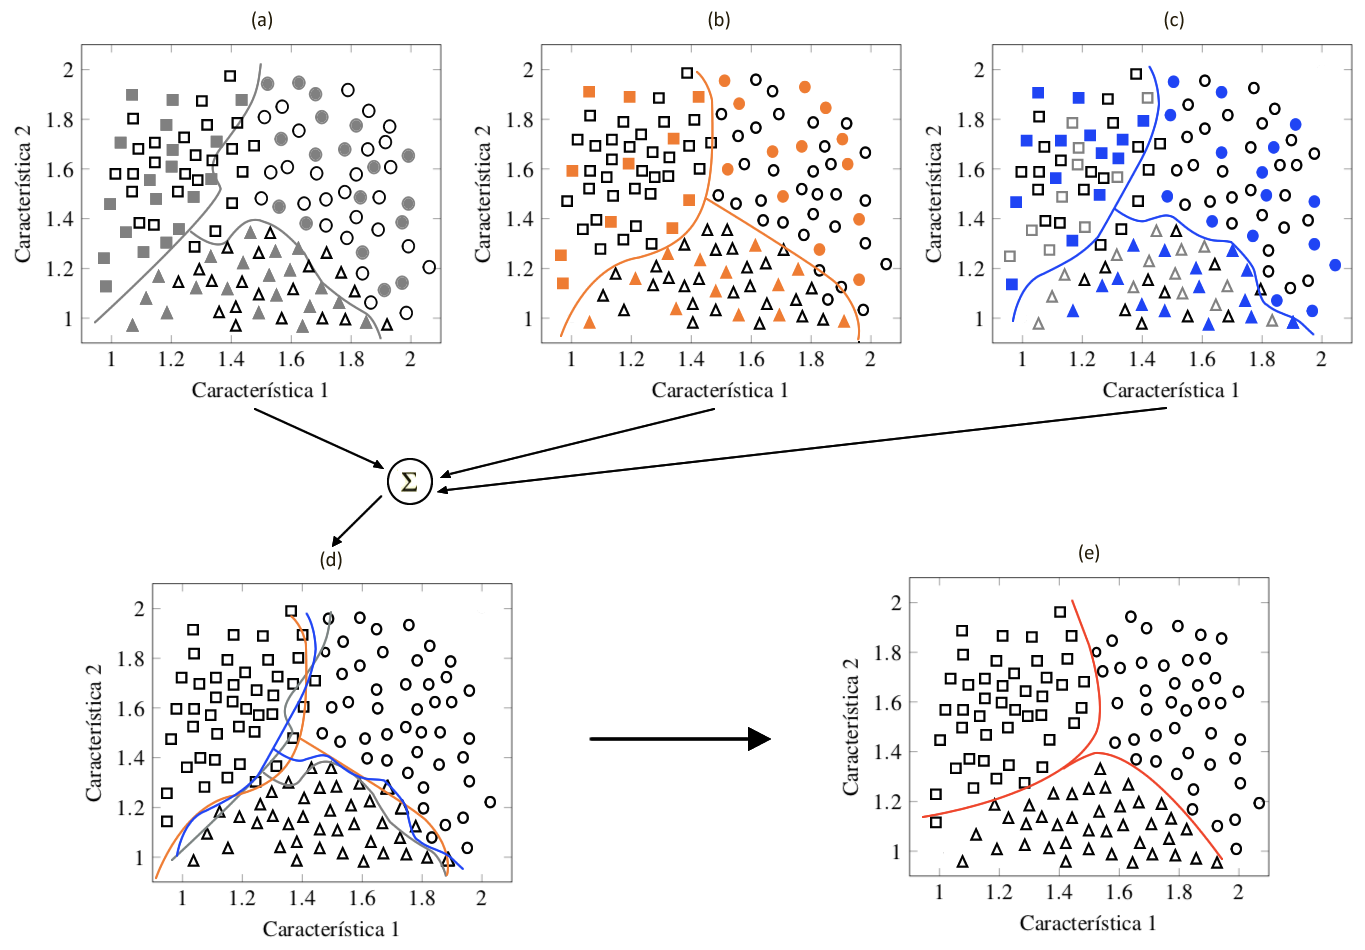
\includegraphics[scale=1.45]{Figuras/Cap4/ensemble.png}
    \begin{center}
    Fonte:
        O autor (2018), adaptado de \cite{zhang2012ensemble}.
    \end{center}
         
        \label{fig:ensemble}
\end{figure}

%FEITO
%\dbh{Sua abordagem de métodos ensemble está muito primitiva! Você precisa ler aqui uns 30 artigos, no mínimo, para melhorar este texto!}

\subsubsection{Teste do modelo}
\label{sec:meto1}

O algoritmo de teste de modelo foi pensado para testar os melhores modelos do algoritmo de seleção de modelo. Nesta fase de teste do modelo, foram utilizados os dados de teste, com objetivo de simular o comportamento real do modelo escolhido. cabe ressaltar que esse é o único momento em todo o trabalho em que os dados de teste são utilizado, a fim de simular o comportamento real do modelo.

O algoritmo proposto para o teste do modelo, neste trabalho, realiza dois \textit{ensemble}, executando várias redes (idealmente um número ímpar de redes), com modelos iguais e inicialização dos pesos diferentes.  Ao executar a previsão, as respostas de cada rede são ordenadas e é escolhida a mediana das respostas como resposta final. 
A técnica do \textit{ensemble} foi aplicada em dois contextos no teste do modelo:

\begin{enumerate}
    \item\textit{Ensemble} de modelo: tendo em vista os resultados da seleção de modelo, foram escolhidos os 7 modelos que apresentaram o menor desvio padrão para o \textit{Ensemble};
    \item \textit{Ensemble} de resultado: para cada modelo do \textit{ensemble} de modelo, são criadas 7 Redes Neurais com mesma arquitetura e inicialização diferente. Todas as 7 Redes Neurais são treinadas e testadas, onde o resultado do modelo passa ser a mediana dos resultados de todas as Redes. A mediana é uma medida mais robusta a aberrações do que a média, daí a sua adoção.
\end{enumerate}

Após executar os dois Ensembles, são obtidos os resultados que serão considerados para esse trabalho. No próximo capítulo serão apresentados os resultados do trabalho, obtidos com as metodologias aqui descritas.